\documentclass[tikz,border=8pt]{standalone}
% Shared UMM figure style (journal-consistent palette + line weights)
\usepackage{tikz}
\usepackage{pgfplots}
\pgfplotsset{compat=1.18}
\usetikzlibrary{arrows.meta,calc,positioning,decorations.pathmorphing,patterns,shapes.geometric,fit,backgrounds}
% Palette: grayscale + single accent (deep teal)
\definecolor{ummAccent}{HTML}{0B6E6E}
\definecolor{ummAccentLight}{HTML}{4A9B9B}
\definecolor{ummDark}{HTML}{1A1A1A}
\definecolor{ummGray}{HTML}{555555}
\definecolor{ummLightGray}{HTML}{AAAAAA}
\definecolor{ummFill}{HTML}{E8F2F2}
\definecolor{ummGas}{HTML}{C45C26}
\definecolor{ummGasLight}{HTML}{F0C4A8}
\definecolor{ummGalaxy}{HTML}{2C3E50}
\definecolor{ummLens}{HTML}{0B6E6E}
\pgfplotsset{
  umm axis/.style={
    axis lines=left,
    axis line style={ummDark, line width=0.8pt},
    tick style={ummDark, line width=0.6pt},
    tick label style={font=\footnotesize, ummDark},
    label style={font=\small, ummDark},
    title style={font=\small\bfseries, ummDark},
    grid=both,
    major grid style={ummLightGray, opacity=0.35, line width=0.3pt},
    minor grid style={ummLightGray, opacity=0.15, line width=0.2pt},
    every axis plot/.append style={line width=1.3pt},
    legend style={font=\footnotesize, draw=ummLightGray, fill=white, fill opacity=0.92, text opacity=1},
    clip=false,
  },
}
\newcommand{\ummLineW}{1.25pt}
\newcommand{\ummLineWthin}{0.9pt}
\tikzset{
  umm arr/.style={-{Latex[length=2.2mm,width=1.6mm]}},
}

\begin{document}
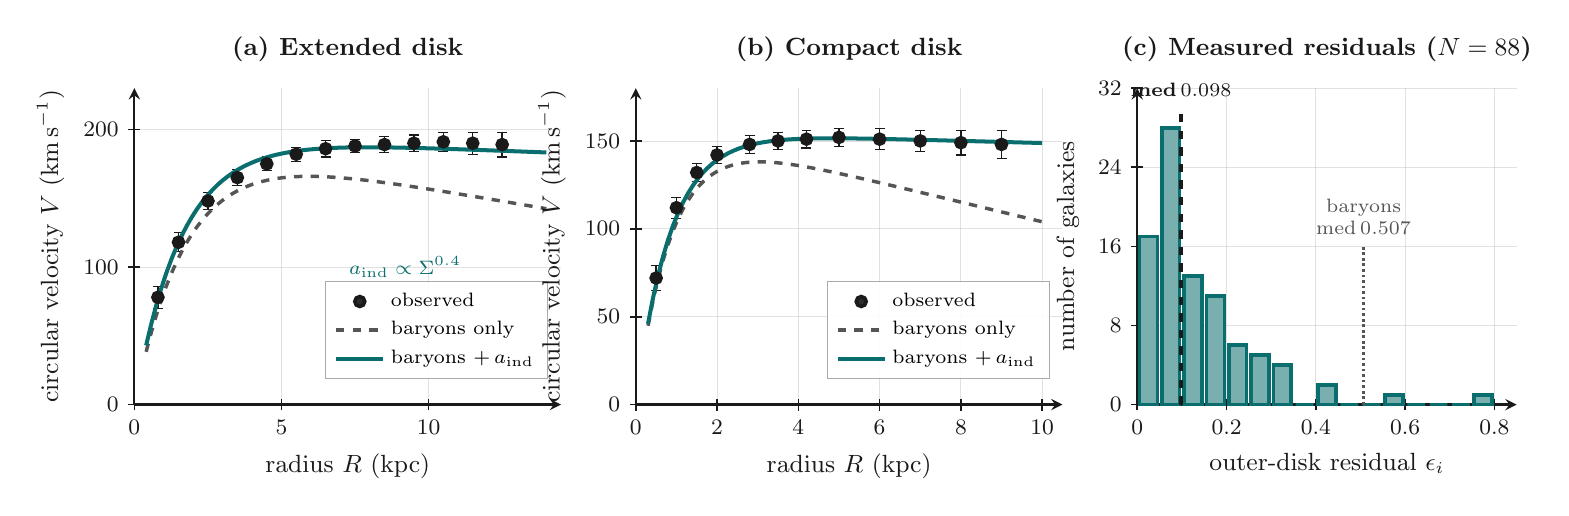
\begin{tikzpicture}
  % ========== Panel (a): rising then flat outer disk ==========
  \begin{axis}[
    umm axis,
    name=axA,
    width=7.0cm,
    height=5.6cm,
    xlabel={radius $R$ (kpc)},
    ylabel={circular velocity $V$ (km\,s$^{-1}$)},
    xmin=0, xmax=14.5,
    ymin=0, ymax=230,
    title={(a) Extended disk},
    legend style={at={(0.97,0.08)}, anchor=south east, font=\scriptsize},
    legend cell align=left,
  ]
    \addplot[only marks, mark=*, mark size=1.8pt, ummDark,
      error bars/.cd, y dir=both, y explicit, error bar style={line width=0.5pt, ummDark}]
      coordinates {
        (0.8, 78) +- (0, 8)
        (1.5, 118) +- (0, 7)
        (2.5, 148) +- (0, 6)
        (3.5, 165) +- (0, 6)
        (4.5, 175) +- (0, 5)
        (5.5, 182) +- (0, 5)
        (6.5, 186) +- (0, 6)
        (7.5, 188) +- (0, 5)
        (8.5, 189) +- (0, 6)
        (9.5, 190) +- (0, 6)
        (10.5, 191) +- (0, 7)
        (11.5, 190) +- (0, 8)
        (12.5, 189) +- (0, 9)
      };
    \addlegendentry{observed}
    \addplot[ummGray, dashed, line width=1.25pt, domain=0.4:14, samples=80]
      {185*(1-exp(-x/1.8))*(1.05-0.28*x/14)};
    \addlegendentry{baryons only}
    \addplot[ummAccent, line width=1.45pt, domain=0.4:14, samples=80]
      {195*(1-exp(-x/1.6))*(1-0.06*x/14)};
    \addlegendentry{baryons $+\,a_{\mathrm{ind}}$}
    \node[font=\scriptsize, ummAccent, align=left] at (axis cs:9.2,100)
      {$a_{\mathrm{ind}}\propto\Sigma^{0.4}$};
  \end{axis}

  % ========== Panel (b): compact disk ==========
  \begin{axis}[
    umm axis,
    name=axB,
    at={($(axA.east)+(0.95cm,0)$)},
    anchor=west,
    width=7.0cm,
    height=5.6cm,
    xlabel={radius $R$ (kpc)},
    ylabel={circular velocity $V$ (km\,s$^{-1}$)},
    xmin=0, xmax=10.5,
    ymin=0, ymax=180,
    title={(b) Compact disk},
    legend style={at={(0.97,0.08)}, anchor=south east, font=\scriptsize},
    legend cell align=left,
  ]
    \addplot[only marks, mark=*, mark size=1.8pt, ummDark,
      error bars/.cd, y dir=both, y explicit, error bar style={line width=0.5pt, ummDark}]
      coordinates {
        (0.5, 72) +- (0, 7)
        (1.0, 112) +- (0, 6)
        (1.5, 132) +- (0, 5)
        (2.0, 142) +- (0, 5)
        (2.8, 148) +- (0, 5)
        (3.5, 150) +- (0, 5)
        (4.2, 151) +- (0, 5)
        (5.0, 152) +- (0, 5)
        (6.0, 151) +- (0, 6)
        (7.0, 150) +- (0, 6)
        (8.0, 149) +- (0, 7)
        (9.0, 148) +- (0, 8)
      };
    \addlegendentry{observed}
    \addplot[ummGray, dashed, line width=1.25pt, domain=0.3:10, samples=80]
      {160*(1-exp(-x/0.9))*(1.0-0.35*x/10)};
    \addlegendentry{baryons only}
    \addplot[ummAccent, line width=1.45pt, domain=0.3:10, samples=80]
      {155*(1-exp(-x/0.85))*(1.0-0.04*x/10)};
    \addlegendentry{baryons $+\,a_{\mathrm{ind}}$};
  \end{axis}

  % ========== Panel (c): residual histogram (measured N=88) ==========
  \begin{axis}[
    umm axis,
    name=axC,
    at={($(axB.east)+(0.95cm,0)$)},
    anchor=west,
    width=6.4cm,
    height=5.6cm,
    xlabel={outer-disk residual $\epsilon_i$},
    ylabel={number of galaxies},
    xmin=0, xmax=0.85,
    ymin=0, ymax=32,
    title={(c) Measured residuals ($N=88$)},
    ytick={0,8,16,24,32},
    xtick={0,0.2,0.4,0.6,0.8},
  ]
    % Histogram bins from analysis/sparc_residuals/results/residuals_main.csv
    % (0.05-wide bins; med $\epsilon_{\rm umm}\approx 0.098$)
    \addplot[ybar, bar width=0.04, ummAccent, fill=ummAccent!55, draw=ummAccent]
      coordinates {
        (0.025, 17)
        (0.075, 28)
        (0.125, 13)
        (0.175, 11)
        (0.225, 6)
        (0.275, 5)
        (0.325, 4)
        (0.375, 0)
        (0.425, 2)
        (0.475, 0)
        (0.525, 0)
        (0.575, 1)
        (0.625, 0)
        (0.675, 0)
        (0.725, 0)
        (0.775, 1)
      };
    % Measured median line
    \draw[ummDark, line width=1.2pt, dashed]
      (axis cs:0.098,0) -- (axis cs:0.098,30);
    \node[font=\scriptsize\bfseries, ummDark, anchor=south]
      at (axis cs:0.098,30.2) {med$\,0.098$};
    % Baryon baseline median mark
    \draw[ummGray, line width=1.0pt, densely dotted]
      (axis cs:0.507,0) -- (axis cs:0.507,16);
    \node[font=\scriptsize, ummGray, anchor=south, align=center]
      at (axis cs:0.507,16.2) {baryons\\med$\,0.507$};
  \end{axis}
\end{tikzpicture}
\end{document}
